\documentclass[11pt]{article}

\usepackage{common}
\usepackage{booktabs}
\usepackage{wrapfig}
\usepackage{titling}
\usepackage{titlesec}
\usepackage{float}
\usepackage[margin=0.99in]{geometry}

\titlespacing\section{0pt}{4pt}{2pt}
\setlength{\parskip}{0.35em}
\setlength{\droptitle}{-5em}
\title{Practical 1: Regression \\ Predicting the Efficiency of Organic Photovoltaics}
\author{Antonio Copete (acopete@cfa.harvard.edu, Camelot.ai Copete) \\
	Fangli Geng (fgeng@g.harvard.edu, Camelot.ai fangligeng) \\
	Xihan Zhang (xihanzhang@hsph.harvard.edu, Camelot.ai Xihan)}
\begin{document}


\maketitle{}


\section{Technical Approach}

We began by performing exploratory analysis on the sample dataset we were given, which consisted of a training set of 1 million molecules with 256 binary predictors, in addition to their SMILES string and the HOMO--LUMO gap we were seeking to predict. The test set consisted of 824,230 molecules with the same set of predictors as well as their SMILES string. The sample code we were given implemented a default Linear Regression model on the full set of 256 predictors, yielding an $R_\textrm{LR}^2 = 0.461 \textrm{ (RMSE}_\textrm{LR} = 0.298)$ over the full training set, and a default Random Forest regression with $R_\textrm{RF}^2 = 0.554 \textrm{ (RMSE}_\textrm{RF} = 0.272)$.

Initial inspection found that out of 256 molecular features, 221 of them were unexpressed (i.e. had $x_i = 0$) for \emph{all} molecules, both in the training set and the test set. Dropping unimportant features would normally call for $K$-fold cross-validation across the training set to ensure those features are consistently unimportant in all cases. However, in the case of null values of certain features for every element of the training set, it is not only legitimate but necessary to drop those features from all further analysis, as fitting along null dimensions would constitute a form of overfitting.

Reducing the sample dataset to 31 expressed features, we performed both regularized and non-regularized linear regression with cross-validation\footnote{After initially trying 3-fold, 5-fold and 10-fold cross-validation, we settled on 5-fold cross-validation as the best compromise between accuracy and computational speed.} and hyperparameter tuning, under the following methods:

\begin{enumerate}

\item Non-regularized linear regression: Yields a mean $R^2 = 0.461$ from 5-fold cross-validation, similar to the original result with 256 predictors.
\item Ridge Regression: Tuning the hyperparamerter $\alpha$ by grid-search cross-validation results in an optimal value of $5.86 \times 10^{-5}$, with a best $R^2 = 0.459$, a result almost identical to non-regularized regression. 
\item Elastic Net: Trying a more general regularization of the form $\alpha_1 L_1 \textrm{(Lasso)} + \alpha_2 L_2$ (Ridge regression), and tuning the $L_1 \textrm{ ratio} \equiv \alpha_1/\alpha_2$ by grid-search cross validation, yields an optimal value of 0.0, which indicates that that a regularization biased towards sparse models, such as the Lasso, might not be the best choice in this case.

\end{enumerate}

The results from linear regression on the sample dataset consistently gave us low predictive value, even when compared to generic random forest regression, which led us into 2 parallel tracks:

%\begin{enumerate}

%\item
1. Feature engineering: 

The RDKit package in Python use the SMILES string to provide an array of information and functions about a molecule, including substructure searching, chemical reaction, enumeration of molecular resonance structures, and several sorts of fingerprints. From our research we decided to extract the \emph{Morgan fingerprint function}, which is widely used with SKLearn in ML and carries the information we considered to be most relevant to the efficiency of organic photovoltaics, such as: (a) Connectivity: Element, numbers of heavy neighbors, numbers of Hs, charge, isotope, inRing; (b) Chemical features: Donor, Acceptor, Aromatic, Halogen, Basic, Acidic; and (c) Taking into account the neighborhood of each atom.

The process takes the ``SMILES'' column from the training and test data and uses RDKit to convert it into molecule objects, followed by gathering of the Morgan fingerprint by use of the command \verb|rdkit.Chem.getmorganfingerprintasbitvect()|, adjusting the parameter \verb|nBits| to 512, 2048 and 4096 to test datasets with various precision levels. After iterating this process for each string, we appended the columns together to form a new input matrix. The size of the dataset greatly varies with precision level, and for this reason we had to slice the datasets into 8 parts in order to accommodate computational constraints.

%\item 
2. Non-linear methods. Among these we concentrated on 2 broad categories:

%\begin{enumerate}

%\item 
(a) Tree-based Ensemble methods: 

Binary predictors are well suited to the branch-like structure of decision trees. Since a deep structure may overfit the training set, we applied ensemble methods to average over the predictions of all trees. The baseline ensemble methods are: (a) Bagging: boostrap multiple training sets to fit multiple trees and reduce the variance. (b) Random Forest: further reduce the variance by randomly picking a subset of $\sqrt{p}$ predictors from the total $p$ at each split. (c) Extremely Randomized Trees: further reduce the variance by selecting cutting points from the subsets totally at random. (d) AdaBoost: use a linear combination of multiple simple trees to reduce the residual step by step.

The baseline models were fitted on the 31 expressed features. A 20\% validation set was used to test the MSE generated by each model. Bagging, Random Forest and Extremely Randomized Trees are quite similar to each other. AdaBoost, which focuses on reducing bias rather than variance, is much weaker. Thus, we selected Random Forest as main model, and tuned the number of estimators (i.e. the total number of trees to average over) to reduce the variance of the model. 5-fold cross-validation was used on 1/8 of the total sample with 2048 newly generated features. 

From the results, we concluded that 13 estimators is sufficient to make the MSE of the test set close to the training set. Given that the total sample size is 8 times that of the test set we used to tune the model, we considered a number of 150 estimators for the whole data set to be reasonable.

The distribution of predictor importances from the baseline random forest is plotted below:

\begin{figure}[H]
\centering
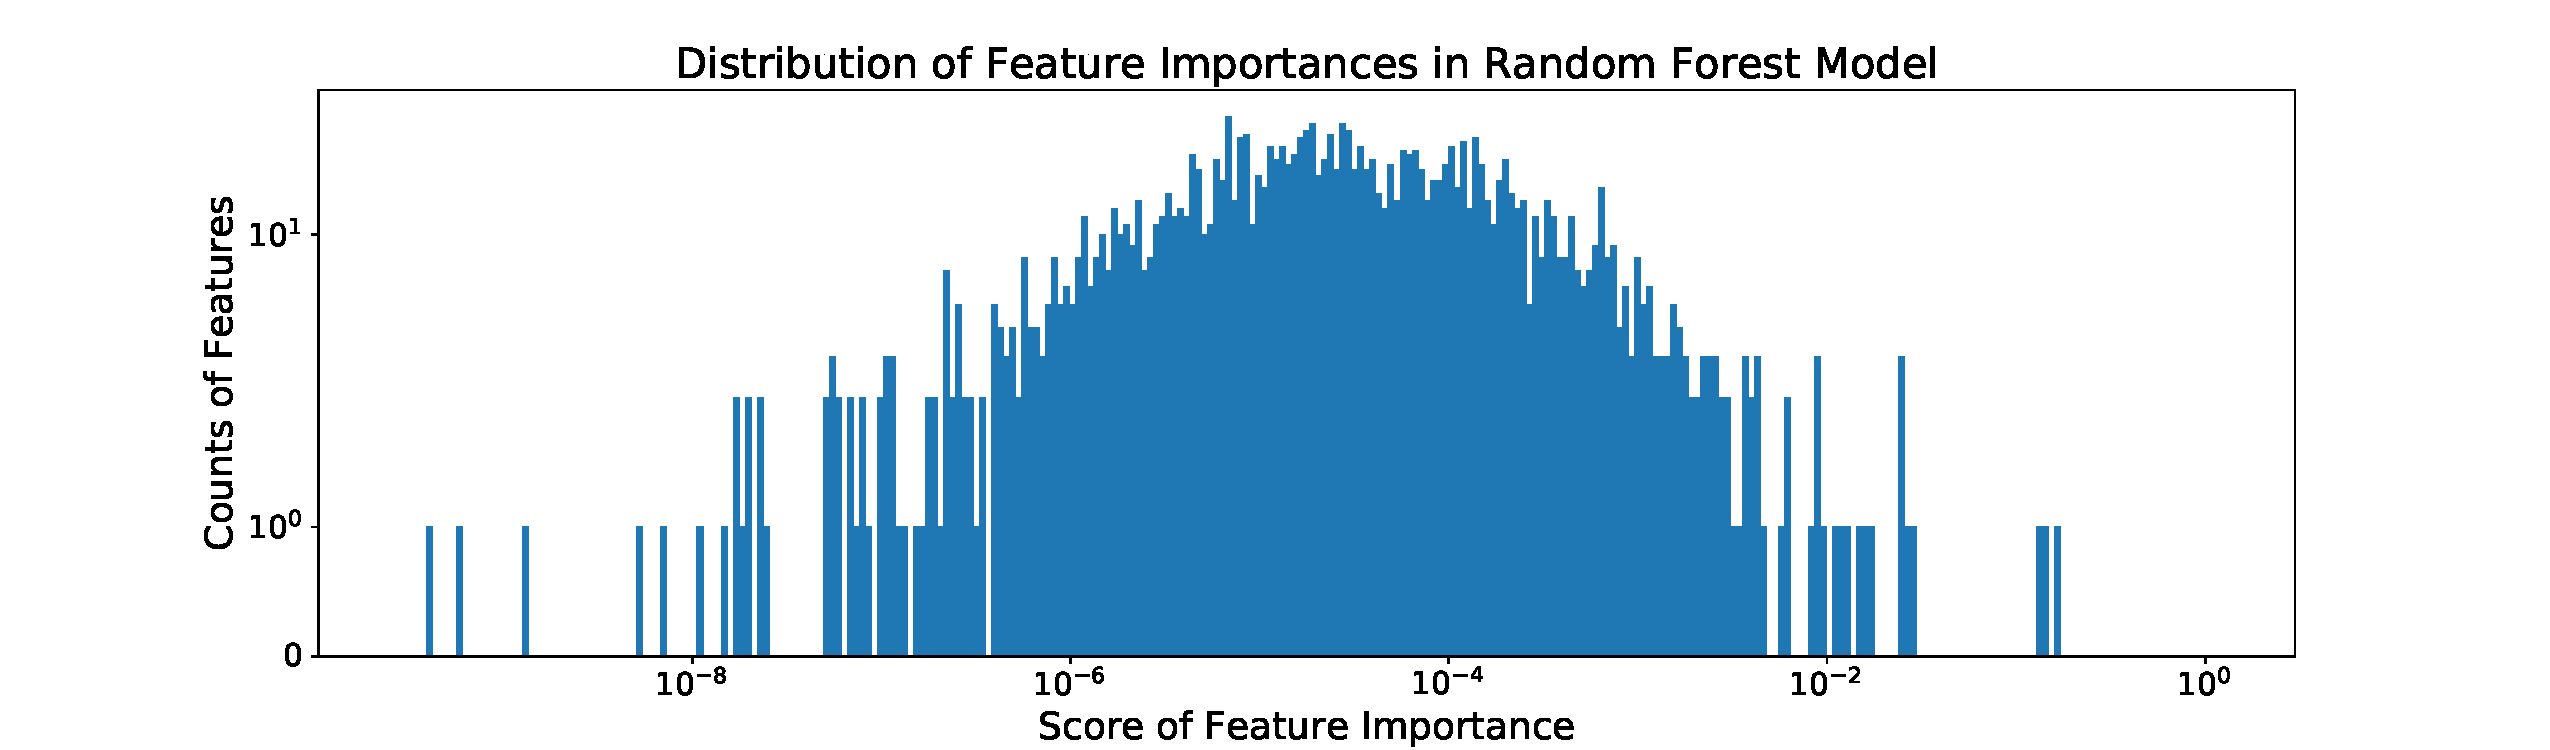
\includegraphics[width=\textwidth]{his_feature_importance}
\caption{Distribution of feature importances from Random Forest}
\label{fig:his_feature_importance}
\end{figure}

Though most predictors have little importance ($10^{-8}$--$10^{-2}$), combining them can result in good precision on the validation set ($R^2 = 0.936$, $\textrm{RMSE}=0.1029$). This made us want to explore further into Deep Learning methods, which consider interactions among features.

%\item 
(b) Deep learning: 

%\end{enumerate}
%\end{enumerate}

In order to model the interactions that would be expected among the broad set of molecular properties extracted from RDKit, we decided to explore the training of simple neural networks and got acquainted with the basics of Deep Learning as a tool to tackle this problem. In all cases, we used an architecture of one or more dense (fully-connected) hidden layers between the input layer of $N$ predictors and the output layer of 1 node for the response we wanted to model. For each node in the hidden layers, we used the widely used ``relu'' function $ f(x) = {\tiny \begin{cases} 0 & \text{if } x \le 0 \\ x & \text{if } x>0 \end{cases}}$ as activation function. We trained the model using the \emph{keras} module in Python, using the \emph{Adam} optimizer for the learning rate, setting aside 20\% of training data for validation. The model fits for the weights of the connections between pairs of nodes in the network, which in the case of 1 hidden layer with $M$ nodes, would result in $(N + 1) \times M$ parameters to be trained.

\begin{wrapfigure}[16]{r}{0.5\textwidth}
\centering
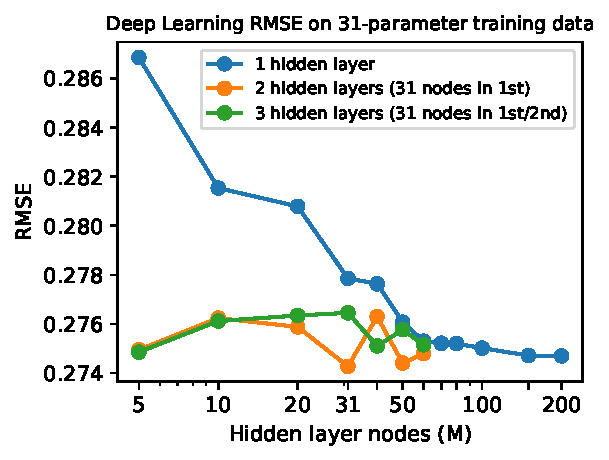
\includegraphics[width=0.5\textwidth]{DL_mse_AC.pdf}
\caption{RMSE of Neural Network architectures}
\label{fig:DL_mse}
\end{wrapfigure}

Taking a trial-and-error approach to the network architecture, we show the results of the validation set RMSE for 3 broad cases, using the 31 expressed features in the sample training dataset: 1) 1 hidden layer with variable number of nodes; 2) 2 hidden layers, with 31 nodes on the first and variable number of nodes on the second; and 3) 3 hidden layers, with 31 nodes on each of the first two, and variable number of nodes on the third.

The result of this experiment showed that the RMSE was not as sensitive to the addition of a second and third layer, as it was to the number of nodes in the first layer of the 1-hidden layer architecture. Given the computational limitations that were expected for a much larger set of features, we used this result to train on the feature-engineered set with only 1-layer models with a limited number of nodes in the same range as the number of predictors.

\section{Results}

\begin{wrapfigure}[15]{r}{0.6\textwidth}
%\begin{figure}[h]
\centering
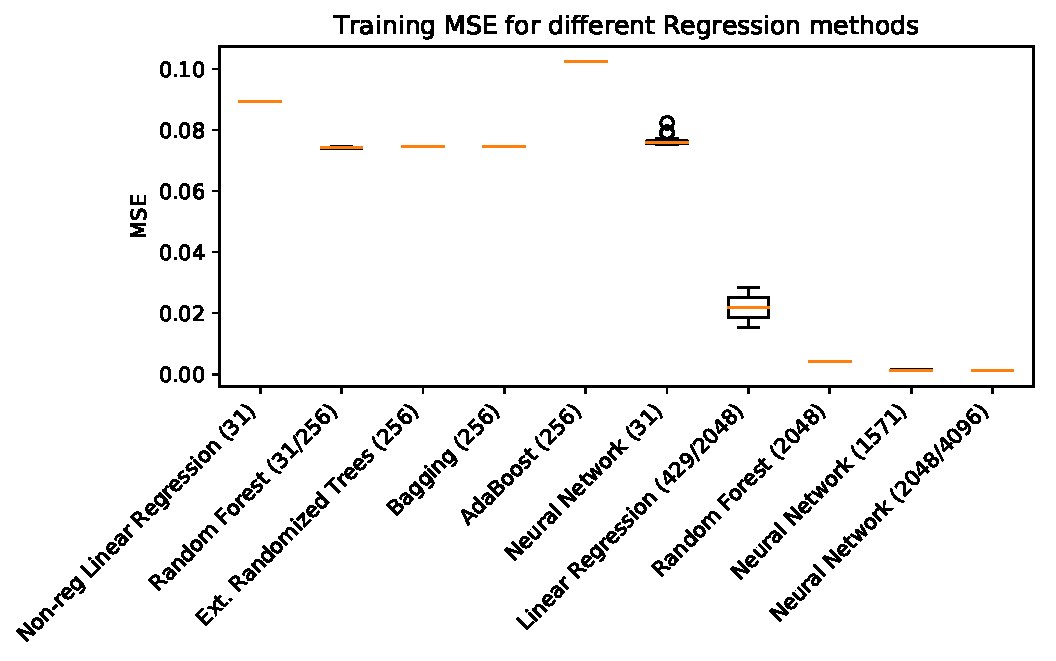
\includegraphics[width=0.58\textwidth]{Results_AC.pdf}
\caption{Overall results for different regression methods and number of predictors}
\label{fig:results}
%\end{figure}
\end{wrapfigure}

Figure \ref{fig:results} summarizes the overall results we obtained from a wide array of regression methods on different sets of features, as described in the Technical Approach section, and roughly listed in the order in which we tried them.

%Table 1 displays the performance of models we tested after we got the new feature information from RDKit. 
%\begin{table}[h]
%\centering
%\begin{tabular}{llr}
% \toprule
% Model &  & RMSE \\
% \midrule
% \textsc{linear regression w/ 2048 features} & & 0.12364\\
% \textsc{linear regression w/ 429 features} & & 0.16869 \\
% \textsc{random forest w/ 2048 features} & & 0.06435 \\
% \textsc{neural network w/ 2048 features w/ 2 layers and 100 units in each layer} & & 0.03564  \\
% \textsc{neural network w/ 2048 features w/ 1000 units} & &0.03553 \\
% \textsc{neural network w/ 4096 features w/ 1024 units} & & 0.03461\\
% \bottomrule
%\end{tabular}
%\caption{\label{tab:results} MSE of models tested using new feature information from RDKit}
%\end{table}

One evident result is the marked improvement in the predictive value of feature-engineered models employing a large number of predictors (429/1571/2048/4096), compared to those from the sample dataset (31/256). Within models of comparable numbers of predictors, linear regression performed relatively poorly, pointing to the non-linear interactions between features that are likely to factor in determining the HOMO--LUMO gaps. Our most accurate results in the Camelot challenge ---as measured by the RMSE on the test set--- came from employing neural network models, and they are summarized in Table~\ref{tab:DLresults}. The 2 best ones ranked 9th ($\textrm{RMSE}= 0.03461$) and 11th ($\textrm{RMSE}= 0.0359$) in the final table, both in the top 10\% of scores.

\begin{table}[h]
\centering
\begin{tabular}{cccrc}
 %\toprule
 Features & Layer 1 & Layer 2 & RMSE & Camelot ranking\\
 \midrule
4096 & 1024 & & 0.03461 & 9 \\
2048 & 100 & 100 & 0.03564 \\
2048 & 1000 & & 0.03553 \\
1571 & 500 & & 0.03645 & 11 \\
 %\bottomrule
\end{tabular}
\caption{\label{tab:DLresults} Best Neural Network model results}
\end{table}

%\begin{enumerate}
%\item Feature set selection

%To select best feature set, we test the performance of the model we have experimented on as mentioned in Technical Approach: 
%\begin{enumerate}
%\item Linear Regression

%We first used 2048 features (which is default in RDKit function) and tested the linear regression. Its results gave us a better result (RMSE 0.1236) than that the best deep learning model (Antonio please put a number here) gave us with 256 features. It indicates the big loss of information using 256 features. \\
%For the purpose of further exploration and reduction of computational burden, we tried to drop the features which have coefficient = 0 from linear regression model results, however, only 1\% of the 2048 features can be dropped. We increased the threshold of dropping data until abs(coefficient)<=0.15, this finally gave a subset with 429 features. We then ran linear regression again with the new subset, but the final RMSE was increased by 30\%. 

%\item Random Forest

%We also ran random forest model with 512 features and 2048 features, but it showed that the 2048 features result was much better than the others. 
%\end{enumerate}

%These two sets of comparison demonstrated that either 429 features selected by linear regression coefficient or 512 features directly given by RDKit fingerprint function was not informative enough. Therefore, we decided to test tune different models with 2048 features, which give us a relatively good amount of information for the molecules energy efficiency prediction. \\

%\item Tuning on neural network

%As discussed in the technical approach part, the experiments using original dataset (256b features) show that neural network with one layer could provide the most accurate results. So we decided to test neural network model With 2048 features. 

%We set up 3 different configurations to conduct the experiments with neural network: 
%\begin{enumerate}
%\item 2 layer neural network with 2048 features and 100 units in each layer; 
%\item 1 layer neural network with 2048 features with 1000 units; 
%\item 1 layer neural network with 4096 features with 1024 units. 
%\end{enumerate}
%Comparing the results between 1st and 2nd experiment, we found the layer number is not as important as unit number, which is consistent with what we found using the smaller number of features. Comparing the result between 2nd and 3rd experiment, we found that 2048 Morgan fingerprint is basically informative enough to predict, and 4096 features in more detail couldn't improve the prediction as much but meanwhile taking a much larger amount of time for computation.

%As 4096 features with 1 layers and 1024 nodes didn't provide the prediction as precise as we expected, we were turning to find additional features and found counted-based fingerprints could be a good option in addition to the bit-based fingerprint we used. Count-based fingerprint count the number of times a feature appears instead of simply that it appears, which could potentially provided new and important information to our prediction. \\

%\item Other methods not realized

%We also wanted to try other algorithms like Principal Component Analysis to select more important features to reduce computational complexity, and to implement neural network models with 2 layer and 2000 nodes to allow more complex interactions between selected important features. However, due to the time constraints we had, we didn't realize those plans. \\

%\item Summary

%As a summary, we found that the linear regression and random forest are good methods to rapidly select useful features. Neural network is much more accurate in non-linear regression, especially with large dataset and rich features condition. \\

%\end{enumerate}

\section{Discussion}

Our approach began with standard exploratory analysis on the sample dataset with 256 features, by fitting Linear Regression and Random Forest as the baseline models. We tried to understand the basic relationships between the data and the given features, and also uncovered a large number of unexpressed molecular features that could be dropped from further analysis. This was followed by more rigorous regularization and cross-validation methods with hyperparameter tuning, which consistently showed a predictive value far below what we wanted to achieve.

Moving onto non-linear methods, we started to experiment with a Deep Learning model with selected important features. We found the Deep Learning model provided the most accurate results so far, as it naturally accounted for interactions among molecular features. Meanwhile, we greatly expanded the number of predictors by drawing the Morgan Fingerprint features from the SMILES strings on RDKit, and produced new training and test datasets with 2048 and 4096 features.

Considering the computational power and time needed to train on the new datasets, we also tried to methodically drop unimportant features, first by dropping unexpressed molecular features as we did before, and then by further refinements based on the feature importances derived from RF Regression models. We tried a limited set of neural network configurations based on our previous experiments, which placed us among the top 10 scores in the Camelot challenge for our best results. From these network architectures we found that the number of layers was not as important as the number of nodes per layer, which is consistent with what we found from the sample dataset. We also found that a set of 2048 Morgan molecular fingerprint features offered the best compromise between accuracy and computational speed.

As for other directions we could have pursued with more time for this Practical, we found that count-based molecular fingerprints could have been a good option in addition to bit-based fingerprints, since they record the number of times a feature appears instead of only whether it appears or not. Also, other statistical approaches such as Principal Component Analysis could have been useful in selecting important features to reduce computational complexity, as well as the use of more complex Neural Network models to account for a richer set of interactions among selected features.

As a summary, we found that the Linear Regression and Random Forest are good methods to rapidly select useful features. Neural Network is much more accurate in non-linear regression, especially with a large dataset and a complex set of features. Finally, we learned that a sophisticated model is no match for having a rich dataset with highly descriptive features to begin with.

\end{document}
